\documentclass[a4paper,10pt]{article}
\usepackage{My_math_package}
\usepackage{pifont}
\usepackage{cancel}

\title{MATH240 Summer 2023} % password: 
\author{Haoran Li}
\date{}

\makeindex[columns=2, title=Index, intoc] % Create the index

\begin{document}\sloppy % Reduce overlong words

\maketitle
\tableofcontents
\newpage



\subsection{Online Assignment 1}

\begin{problem}
Rewrite the following linear systems as augmented matrices and then solve them, show all your work
\begin{enumerate}
\item $\begin{cases}
5x_1+x_2=2\\
3x_1-x_2=6
\end{cases}$
\item $\begin{cases}
x_1+x_2+x_3=6\\
x_1-x_2+x_3=2\\
-x_1+x_2+x_3=4
\end{cases}$
\end{enumerate}
\end{problem}

\begin{solution}
\begin{enumerate}
\item The augmented matrix is
\begin{align*}
&\begin{bmatrix}
5&1&2\\
3&-1&6
\end{bmatrix}\xsim{5R2}\begin{bmatrix}
5&1&2\\
15&-5&30
\end{bmatrix}\xsim{R2\rightarrow R2-3R1}\begin{bmatrix}
5&1&2\\
0&-8&24
\end{bmatrix}\xsim{R2/(-8)}\begin{bmatrix}
5&1&2\\
0&1&-3
\end{bmatrix}\\
&\xsim{R1\rightarrow R1-R2}\begin{bmatrix}
5&0&5\\
0&1&-3
\end{bmatrix}\xsim{R1/5}\begin{bmatrix}
1&0&1\\
0&1&-3
\end{bmatrix}
\end{align*}
Thus the solution to this linear system is $\begin{cases}
x_1=1\\x_2=-3
\end{cases}$
\item The augmented matrix is
\begin{align*}
&\begin{bmatrix}
1&1&1&6\\
1&-1&1&2\\
-1&1&1&4
\end{bmatrix}\xsim{\substack{R2\rightarrow R2-R1\\R3\rightarrow R3+R1}}\begin{bmatrix}
1&1&1&6\\
0&-2&0&-4\\
0&2&2&10
\end{bmatrix}\xsim{R3\rightarrow R3+R2}\begin{bmatrix}
1&1&1&6\\
0&-2&0&-4\\
0&0&2&6
\end{bmatrix}\\
&\xsim{\substack{R2/(-2)\\R3/3}}\begin{bmatrix}
1&1&1&6\\
0&1&0&2\\
0&0&1&3
\end{bmatrix}\xsim{\substack{R1\rightarrow R1-R2-R3}}\begin{bmatrix}
1&0&0&1\\
0&1&0&2\\
0&0&1&3
\end{bmatrix}
\end{align*}
Thus the solution to this linear system is $\begin{cases}
x_1=1\\x_2=2\\x_3=3
\end{cases}$
\end{enumerate}
\end{solution}

\begin{problem}
How many solutions does the following linear systems of equations have
\begin{enumerate}
\item $\begin{cases}
5x_1+7x_2=3\\
-10x_1-14x_2=-3
\end{cases}$
\item $\begin{cases}
2x_1-x_2=4\\
x_1-\frac{1}{2}x_2=2
\end{cases}$
\end{enumerate}
\end{problem}

\begin{solution}
\begin{enumerate}
\item The augmented matrix is
\begin{align*}
&\begin{bmatrix}
5&7&3\\
-10&-14&-3
\end{bmatrix}\xsim{R2\rightarrow R2+2R1}\begin{bmatrix}
5&7&3\\
0&0&3
\end{bmatrix}
\end{align*}
Since the last column has pivot, by Theorem~\ref{14:16-06/03/2022}, this linear system has no solutions
\item \begin{align*}
&\begin{bmatrix}
2&-1&4\\
1&-\frac{1}{2}&2
\end{bmatrix}\xsim{R2\rightarrow R2-\frac{1}{2}R1}\begin{bmatrix}
2&-1&4\\
0&0&0
\end{bmatrix}
\end{align*}
Since the last column has no pivot and there is a free variable $x_2$, by Theorem~\ref{14:16-06/03/2022}, this linear system has infinitely solutions
\end{enumerate}
\end{solution}

\begin{problem}
Consider the following matrix
$$
A=\begin{bmatrix}
1&2&2&3&1\\
0&0&-1&2&1\\
0&0&0&2&4\\
\end{bmatrix}
$$
\begin{enumerate}
\item Which columns are the pivot columns of $A$?
\item Write down the RREF of the this matrix
\end{enumerate}
\end{problem}

\begin{solution}
\begin{enumerate}
\item The pivot columns of $A$ are columns 1,3,4.
\item 
\begin{align*}
&A\xsim{\substack{R2/(-1)\\R3/2}}\begin{bmatrix}
1&2&2&3&1\\
0&0&1&-2&-1\\
0&0&0&1&2\\
\end{bmatrix}\xsim{\substack{R1\rightarrow R1-3R3\\R2\rightarrow R2+2R3}}\begin{bmatrix}
1&2&2&0&-5\\
0&0&1&0&3\\
0&0&0&1&2\\
\end{bmatrix}\xsim{R1\rightarrow R1-2R2}\begin{bmatrix}
1&2&0&0&-11\\
0&0&1&0&3\\
0&0&0&1&2\\
\end{bmatrix}
\end{align*}
\end{enumerate}
\end{solution}

\begin{problem}
Determine which of the following statements are true
\begin{enumerate}
\item The following matrix is of row reduced echelon form
$$
\begin{bmatrix}
1&2&2&3&1\\
0&0&0&2&4\\
0&0&-1&2&1\\
\end{bmatrix}
$$
\item The following two matrices are equivalent
$$
\begin{bmatrix}
1&-1&1&3&2\\
2&4&1&2&4\\
1&1&-3&2&1\\
\end{bmatrix}\sim
\begin{bmatrix}
1&2&2&3&1\\
0&0&0&2&4\\
0&0&-1&2&1\\
\end{bmatrix}
$$
\end{enumerate}
\end{problem}

\begin{solution}
\begin{enumerate}
\item False. $(3,3)$, $(2,4)$-th entries are pivots which breaks the ``staircase shape"
\begin{tikzpicture}
\node at (0,0) {$\begin{bmatrix}
\textcolor{red}{1}&2&2&3&1\\
0&0&0&\textcolor{red}{2}&4\\
0&0&\textcolor{red}{-1}&2&1\\
\end{bmatrix}$};
\draw[thick, red] (-1.4,0.2)--(0.4,0.2)--(0.4,-0.2)--(-0.4,-0.2)--(-0.4,-0.6)--(1.4,-0.6);
\end{tikzpicture}
\item False. Because
\begin{align*}
&\begin{bmatrix}
1&-1&1&3&2\\
2&4&1&2&4\\
1&1&-3&2&1\\
\end{bmatrix}\xsim{\substack{R2\rightarrow R2-2R1\\R3-R1}}\begin{bmatrix}
1&-1&1&3&2\\
0&6&-1&-4&0\\
0&2&-4&-1&-1\\
\end{bmatrix}\\
&\xsim{R2\rightarrow R2-3R3}\begin{bmatrix}
1&-1&1&3&2\\
0&0&11&14&3\\
0&2&-4&-1&-1\\
\end{bmatrix}\xsim{R2\leftrightarrow R3}\begin{bmatrix}
1&-1&1&3&2\\
0&2&-4&-1&-1\\
0&0&11&14&3\\
\end{bmatrix}
\end{align*}
has pivot columns 1,2,3, and
\begin{align*}
\begin{bmatrix}
1&2&2&3&1\\
0&0&0&2&4\\
0&0&-1&2&1\\
\end{bmatrix}\xsim{R2\leftrightarrow R3}\begin{bmatrix}
1&2&2&3&1\\
0&0&-1&2&1\\
0&0&0&2&4\\
\end{bmatrix}
\end{align*}
has pivot columns 1,3,4. By Theorem~\ref{18:46-06/08/2022}, they are not equivalent, otherwise they would have the same RREF, which implies same pivot columns.
\end{enumerate}
\end{solution}

\begin{problem}
Determine the value(s) of $h$ such that the matrix is the augmented matrix of a consistent linear system
$
\begin{bmatrix}
1&h&1\\
2&4&4\\
\end{bmatrix}
$
\end{problem}

\begin{solution}
First consider
\[
\begin{bmatrix}
1&h&1\\
2&4&4\\
\end{bmatrix}\xsim{R2\rightarrow R2-2R1}\begin{bmatrix}
1&h&1\\
0&4-2h&2\\
\end{bmatrix}
\]
By Theorem~\ref{14:16-06/03/2022}, the linear system has solutions $\iff$ the last column is not a pivot column $\iff 4-2h\neq0\iff h\neq2$
\end{solution}

\begin{problem}
Do the three lines $x_1-4x_2 = 1$, $2x_1-x_2 =-3$, and $-x_1 - 3x_2 = 4$ have a common point of intersection? Explain.
\end{problem}

\begin{solution}
Note that a common point of intersection would be a solution to the linear system \systeme{x_1-4x_2 = 1, 2x_1-x_2 =-3, -x_1 - 3x_2 = 4}, consider its augmented matrix
\begin{align*}
&\begin{bmatrix}
1&-4&1\\
2&-1&-3\\
-1&-3&4
\end{bmatrix}\xsim{\substack{R2\rightarrow R2-2R1\\R3\rightarrow R3+R1}}\begin{bmatrix}
1&-4&1\\
0&7&-5\\
0&-7&5
\end{bmatrix}\xsim{R3\rightarrow R3+R2}\begin{bmatrix}
1&-4&1\\
0&7&-5\\
0&0&0
\end{bmatrix}
\end{align*}
By Theorem~\ref{14:16-06/03/2022}, since the last column is not a pivot column, the linear system is consistent, i.e. these three lines has comon point(s) of intersection.
\end{solution}

\subsection{Online Assignment 2}

\begin{problem}
Consider the following statements
\begin{enumerate}
\item For any four distinct vectors $\mathbf v_1,\mathbf v_2,\mathbf v_3,\mathbf v_4$ in $\mathbb R^3$, $\operatorname{Span}\{\mathbf v_1,\mathbf v_2,\mathbf v_3,\mathbf v_4\}=\mathbb R^3$
\item Suppose we know that the augmented matrix of the linear system
\[
\begin{cases}
a_1x_1+a_2x_2+a_3x_3=d_1\\
b_1x_1+b_2x_2+b_3x_3=d_2\\
c_1x_1+c_2x_2+c_3x_3=d_3
\end{cases}
\]
has two pivot columns, then how many solutions could the linear system have?
\item Consider matrix equation $A\mathbf x=\mathbf 0$ where $A$ is a 3 by 4 matrix, then it always has more than one solution (obviously $\mathbf x=\mathbf0$ will be a solution)
\end{enumerate}
\end{problem}

\begin{solution}
\begin{enumerate}
\item False. A counter-example would be $\mathbf v_1=\begin{bmatrix}
1\\0\\0
\end{bmatrix}$,$\mathbf v_2=\begin{bmatrix}
0\\1\\0
\end{bmatrix}$,$\mathbf v_3=\begin{bmatrix}
1\\1\\0
\end{bmatrix}$,$\mathbf v_4=\begin{bmatrix}
1\\-1\\0
\end{bmatrix}$, then $\mathbf b=\begin{bmatrix}
0\\0\\1
\end{bmatrix}$ is not in $\Span\{\mathbf v_1,\mathbf v_2,\mathbf v_3,\mathbf v_4\}$ since
\[
\begin{bmatrix}
1&0&1&1&0\\
0&1&1&-1&0\\
0&0&0&0&1
\end{bmatrix}
\]
has pivot in the last row, and apply Theorem~\ref{14:16-06/03/2022}
\item The number of solutions could be none or infinitely many. There are in total 6 possible cases (apply Theorem~\ref{14:16-06/03/2022})
\begin{enumerate}[label=Case \roman*:]
\item The pivot columns are 1,2, then augmented matrix is equivalent to the RREF matrix $\begin{bmatrix}
1&0&*&*\\
0&1&*&*\\
0&0&0&0\\
\end{bmatrix}$, so the linear system have infinitely many solutions and $x_3$ is a free variable.
\item The pivot columns are 1,3, then augmented matrix is equivalent to the RREF matrix $\begin{bmatrix}
1&*&0&*\\
0&0&1&*\\
0&0&0&0\\
\end{bmatrix}$, so the linear system have infinitely many solutions. and $x_2$ is a free variable.
\item The pivot columns are 1,4, then augmented matrix is equivalent to the RREF matrix $\begin{bmatrix}
1&*&*&0\\
0&0&0&1\\
0&0&0&0\\
\end{bmatrix}$, so the linear system have no solutions.
\item The pivot columns are 2,3, then augmented matrix is equivalent to the RREF matrix $\begin{bmatrix}
0&1&0&*\\
0&0&1&*\\
0&0&0&0\\
\end{bmatrix}$, so the linear system have infinitely many solutions. and $x_1$ is a free variable.
\item The pivot columns are 2,4, then augmented matrix is equivalent to the RREF matrix $\begin{bmatrix}
0&1&*&0\\
0&0&0&1\\
0&0&0&0\\
\end{bmatrix}$, so the linear system have no solutions.
\item The pivot columns are 3,4, then augmented matrix is equivalent to the RREF matrix $\begin{bmatrix}
0&0&1&0\\
0&0&0&1\\
0&0&0&0\\
\end{bmatrix}$, so the linear system have no solutions.
\end{enumerate}
\item
\begin{align*}
&\begin{bmatrix}
*&*&*&*&0\\
*&*&*&*&0\\
*&*&*&*&0
\end{bmatrix}=\begin{bmatrix}
A&\mathbf0
\end{bmatrix}\sim\begin{bmatrix}
U&\mathbf0
\end{bmatrix}
\end{align*}
Since it doesn't have a pivot in the last column, it must have a solution (indeed at least the trivial solution) by Theorem~\ref{14:16-06/03/2022}, and since $A$ has more columns that rows, there must be a free variable, therefore it has infinitely many solutions
\end{enumerate}
\end{solution}

\begin{problem}
Answer the following questions
\begin{enumerate}
\item Determine whether $\mathbf b=\begin{bmatrix}1\\1\\2\end{bmatrix}$ is in the span of $\left\{\mathbf v_1=\begin{bmatrix}1\\0\\2\end{bmatrix},\mathbf v_2=\begin{bmatrix}2\\2\\6\end{bmatrix},\mathbf v_3=\begin{bmatrix}-1\\-2\\-4\end{bmatrix}\right\}$, why?
\item Assume $\mathbf w=\begin{bmatrix}1\\0\\2\end{bmatrix}$, $\mathbf v_1=\begin{bmatrix}1\\1\\0\end{bmatrix}$, $\mathbf v_2=\begin{bmatrix}1\\4\\-4\end{bmatrix}$, $\mathbf v_3=\begin{bmatrix}0\\1\\-1\end{bmatrix}$. Find constants $c_1,c_2$ such that $\mathbf w=c_1\mathbf v_1+c_2\mathbf v_2+2\mathbf v_3$. Show your work on how you found $c_1,c_2$.
\item Suppose 
\[
A=\begin{bmatrix}
1   &  3    & 0&     3\\
-1   & -1  &  -1 &    1\\
0    &-4  &   2   & -8\\
2     &0&     3   & -1
\end{bmatrix}
\]
Is it true that for any vector $\mathbf b$ in $\mathbb R^4$, matrix equation $A\mathbf x=\mathbf b$ always has solution(s)? If it is, please give your reason. If it is not, please find one such $\mathbf b$ and justify your answer.
\end{enumerate}
\end{problem}

\begin{solution}
\begin{enumerate}
\item Consider 
\begin{align*}
&\begin{bmatrix}
\mathbf v_1&\mathbf v_2&\mathbf v_3&\mathbf b
\end{bmatrix}=\begin{bmatrix}
A&\mathbf b
\end{bmatrix}=\begin{bmatrix}
1&2&-1&1\\
0&2&-2&1\\
2&6&-4&2
\end{bmatrix}\xsim{R3\rightarrow R3-2R1}\begin{bmatrix}
1&2&-1&1\\
0&2&-2&1\\
0&2&-2&0
\end{bmatrix}\\
&\xsim{R3\rightarrow R3-R2}\begin{bmatrix}
1&2&-1&1\\
0&2&-2&1\\
0&0&0&-1
\end{bmatrix}
\end{align*}
By Theorem~\ref{14:16-06/03/2022}, $A\mathbf x=\mathbf b$ has no solution, i.e. $\mathbf b$ is not in $\Span\{\mathbf v_1,\mathbf v_2,\mathbf v_3\}$. So we should consider augmented matrix
\begin{align*}
&\begin{bmatrix}
1&1&1\\
1&4&-2\\
0&-4&4
\end{bmatrix}\xsim{R2\rightarrow R2-R1}\begin{bmatrix}
1&1&1\\
0&3&-3\\
0&-4&4
\end{bmatrix}\xsim{R2/3}\begin{bmatrix}
1&1&1\\
0&1&-1\\
0&-4&4
\end{bmatrix}\xsim{\substack{R3\rightarrow R3+4R2\\R1\rightarrow R1-R2}}\begin{bmatrix}
1&0&2\\
0&1&-1\\
0&0&0
\end{bmatrix}
\end{align*}
Hence $c_1=2$, $c_2=-1$.
\item It is equivalent to solving $c_1\mathbf v_1+c_2\mathbf v_2=\mathbf w-2\mathbf v_3=\begin{bmatrix}
1\\-2\\4
\end{bmatrix}$
\item
\begin{align*}
&A\xsim{\substack{R2\rightarrow R2+R1\\R4\rightarrow R4-2R1}}\begin{bmatrix}
1   &  3    & 0&     3\\
0   & 2  &  -1 &    4\\
0    &-4  &   2   & -8\\
0     &-6 &     3   & -7
\end{bmatrix}\xsim{\substack{R3\rightarrow R3+2R2\\R4\rightarrow R4+3R2}}\begin{bmatrix}
1   &  3    & 0&     3\\
0   & 2  &  -1 &    4\\
0    &0  &   0   & 0\\
0     &0 &    0  & 5
\end{bmatrix}\xsim{R3\leftrightarrow R4}\begin{bmatrix}
1   &  3    & 0&     3\\
0   & 2  &  -1 &    4\\
0     &0 &    0  & 5\\
0    &0  &   0   & 0
\end{bmatrix}
\end{align*}
Which doesn't have pivot in the last row, so $A\mathbf x=\mathbf b$ doesn't always have a solution by Theorem~\ref{16:05-06/06/2022}. To find one such $\mathbf b$, you can just try (Since the range of the linear transformation $\mathbf x\mapsto A\mathbf x$ is the span of the columns of $A$ which is a hyperplane in $\mathbb R^4$, so choosing an arbitrary point is most likely not on that hyperplane, i.e. $A\mathbf x=\mathbf b$ not solvable!). Here we just try $\mathbf b=\begin{bmatrix}
0\\0\\1\\0
\end{bmatrix}$, then
\begin{align*}
&\begin{bmatrix}
A&\mathbf b
\end{bmatrix}=\begin{bmatrix}
1   &  3    & 0&     3&0\\
-1   & -1  &  -1 &    1&0\\
0    &-4  &   2   & -8&1\\
2     &0&     3   & -1&0
\end{bmatrix}\xsim{\substack{R2\rightarrow R2+R1\\R4\rightarrow R4-2R1}}\begin{bmatrix}
1   &  3    & 0&     3&0\\
0   & 2  &  -1 &    4&0\\
0    &-4  &   2   & -8&1\\
0     &-6 &     3   & -7&0
\end{bmatrix}\\
&\xsim{\substack{R3\rightarrow R3+2R2\\R4\rightarrow R4+3R2}}\begin{bmatrix}
1   &  3    & 0&     3&0\\
0   & 2  &  -1 &    4&0\\
0    &0  &   0   & 0&1\\
0     &0 &    0  & 5&0
\end{bmatrix}\xsim{R3\leftrightarrow R4}\begin{bmatrix}
1   &  3    & 0&     3&0\\
0   & 2  &  -1 &    4&0\\
0     &0 &    0  & 5&0\\
0    &0  &   0   & 0&1
\end{bmatrix}
\end{align*}
\end{enumerate}
\end{solution}

\subsection{Online Assignment 3}

\begin{problem}
Suppose $\mathbf v_1,\mathbf v_2,\mathbf v_3$ are vectors in $\mathbb R^4$, if $\{\mathbf v_1,\mathbf v_2\}$ is linearly independent, $\{\mathbf v_2,\mathbf v_3\}$ is linearly independent, and $\{\mathbf v_1,\mathbf v_3\}$ is linearly independent, then $\{\mathbf v_1,\mathbf v_2,\mathbf v_3\}$ is linearly independent
\end{problem}

\begin{solution}
False. For example $\left\{\mathbf v_1=\begin{bmatrix}
1\\0\\0\\0
\end{bmatrix},\mathbf v_2=\begin{bmatrix}
0\\1\\0\\0
\end{bmatrix},\mathbf v_3=\begin{bmatrix}
1\\1\\0\\0
\end{bmatrix}\right\}$
\end{solution}

\begin{problem}
Suppose $A$ is a $m$ by $n$ matrix, and the matrix equation $A\mathbf x=\mathbf b$ always has solution for any vector $\mathbf b$ in $\mathbb R^m$, the columns of $A$ are linearly independent
\end{problem}

\begin{solution}
False. There could be free variables
\end{solution}

\begin{problem}
Solve the linear system $\begin{cases}
x_1+x_2+x_3+x_4=1\\
2x_1-x_2+x_3-x_4=-1\\
\end{cases}$ and express its solution set in parametric vector form
\end{problem}

\begin{solution}
Write the augmented matrix
\begin{align*}
&\begin{bmatrix}
1&1&1&1&1\\
2&-1&1&-1&-1
\end{bmatrix}\xsim{R2\rightarrow R2-2R1}\begin{bmatrix}
1&1&1&1&1\\
0&-3&-1&-3&-3
\end{bmatrix}\xsim{R2/(-3)}\begin{bmatrix}
1&1&1&1&1\\
0&1&\frac{1}{3}&1&1
\end{bmatrix}\\
&\xsim{R1\rightarrow R1-R2}\begin{bmatrix}
1&0&\frac{2}{3}&0&0\\
0&1&\frac{1}{3}&1&1
\end{bmatrix}
\end{align*}
So the solution set is
\[
\systeme*{x_1+\frac{2}{3}x_3=0, x_2+\frac{1}{3}x_3+x_4=1}\Rightarrow\begin{cases}
x_1=-\frac{2}{3}x_3\\
x_2=1-\frac{1}{3}x_3-x_4\\
x_3\text{ is free}\\
x_4\text{ is free}
\end{cases}
\]
Its parametric vector form is
\[
\begin{bmatrix}
x_1\\x_2\\x_3\\x_4
\end{bmatrix}=\begin{bmatrix}
-\frac{2}{3}x_3\\1-\frac{1}{3}x_3-x_4\\x_3\\x_4
\end{bmatrix}=\begin{bmatrix}
0\\1\\0\\0
\end{bmatrix}+\begin{bmatrix}
-\frac{2}{3}x_3\\-\frac{1}{3}x_3\\x_3\\0
\end{bmatrix}+\begin{bmatrix}
0\\-x_4\\0\\x_4
\end{bmatrix}=\begin{bmatrix}
0\\1\\0\\0
\end{bmatrix}+x_3\begin{bmatrix}
-\frac{2}{3}\\-\frac{1}{3}\\1\\0
\end{bmatrix}+x_4\begin{bmatrix}
0\\-1\\0\\1
\end{bmatrix}
\]
\end{solution}

\begin{problem}
Suppose $\mathbf v_1=\begin{bmatrix}
1\\0\\1
\end{bmatrix}$, $\mathbf v_2=\begin{bmatrix}
0\\-1\\1
\end{bmatrix}$, $\mathbf v_3=\begin{bmatrix}
-2\\3\\-11
\end{bmatrix}$, $\mathbf v_4=\begin{bmatrix}
0\\0\\-3
\end{bmatrix}$. Is $\{\mathbf v_1,\mathbf v_2,\mathbf v_3,\mathbf v_4\}$ linearly independent? If so, please give your reason, if not, please find a linear dependence (i.e. some linear combination $c_1\mathbf v_1+c_2\mathbf v_2+c_2\mathbf v_3+c_4\mathbf v_4=0$, $c_1,c_2,c_3,c_4$ not all zero)
\end{problem}

\begin{solution}
Consider
\begin{align*}
&\begin{bmatrix}
\mathbf v_1&\mathbf v_2&\mathbf v_3&\mathbf v_4&\mathbf0
\end{bmatrix}=\begin{bmatrix}
1&0&-2&0&0\\
0&-1&3&0&0\\
1&1&-11&-3&0
\end{bmatrix}\xsim{R3\rightarrow R3-R1}\begin{bmatrix}
1&0&-2&0&0\\
0&-1&3&0&0\\
0&1&-9&-3&0
\end{bmatrix}\\
&\xsim{R3\rightarrow R3+R2}\begin{bmatrix}
1&0&-2&0&0\\
0&-1&3&0&0\\
0&0&-6&-3&0
\end{bmatrix}\xsim{\substack{(-1)R2\\R3/(-6)}}\begin{bmatrix}
1&0&-2&0&0\\
0&1&-3&0&0\\
0&0&1&\frac{1}{2}&0
\end{bmatrix}\xsim{\substack{R1\rightarrow R1+2R3\\R2\rightarrow R2+3R3}}\begin{bmatrix}
1&0&0&1&0\\
0&1&0&\frac{3}{2}&0\\
0&0&1&\frac{1}{2}&0
\end{bmatrix}
\end{align*}
So the solution set is
\[
\begin{cases}
x_1=-x_4\\x_2=-\frac{3}{2}x_4\\x_3=-\frac{1}{2}x_4\\x_4\text{ is free}
\end{cases}
\]
We can choose $x_4=-2$, then $x_1=2, x_2=3, x_3=1$ so that we know $2\mathbf v_1+3\mathbf v_2+\mathbf v_3-2\mathbf v_4=\mathbf0$ is a linear dependence.
\end{solution}

\begin{problem}
Suppose linear transformation $T:\mathbb R^2\to\mathbb R^2$ rotates the plane $\mathbb R^2$ counter-clockwise by $120^\circ$, what is the standard matrix for the this linear transformation?
\end{problem}

\begin{solution}
the standard matrix for $T$ is
\[
A=\begin{bmatrix}
T(\mathbf e_1)&T(\mathbf e_2)
\end{bmatrix}=\begin{bmatrix}
-\frac{1}{2}&-\frac{\sqrt{3}}{2}\\
\frac{\sqrt{3}}{2}&-\frac{1}{2}
\end{bmatrix}
\]
\begin{center}
\begin{tikzpicture}[scale=2]
\def\XMAX{1.5};\def\YMAX{1.5};
\draw[help lines, color=gray!30, dashed] (-\XMAX,-\YMAX) grid (\XMAX,\YMAX);
\draw[->, color=gray!80] (-\XMAX,0)--(\XMAX,0) node[right]{$x_1$};
\draw[->, color=gray!80] (0,-\YMAX)--(0,\YMAX) node[above]{$x_2$};
\draw[opacity=0.6, red, dashed] (0,0) circle (1);
\coordinate (a) at (1,0); \node at (a)[below right]{$\mathbf e_1$}; \draw[->, thick] (0,0)--(a);
\coordinate (b) at (0,1); \node at (b)[above right]{$\mathbf e_2$}; \draw[->, thick] (0,0)--(b);
\coordinate (c) at ($cos(120)*(1,0)+sin(120)*(0,1)$); \node at (c)[above left]{\textcolor{purple}{$T(\mathbf e_1)$}}; \draw[->, purple, thick] (0,0)--(c);
\coordinate (d) at ($cos(210)*(1,0)+sin(210)*(0,1)$); \node at (d)[below left]{\textcolor{blue}{$T(\mathbf e_2)$}}; \draw[->, blue, thick] (0,0)--(d);
\draw[opacity=0.6, purple, dashed] (c)--($cos(120)*(1,0)$);
\draw[opacity=0.6, purple, dashed] (c)--($sin(120)*(0,1)$);
\draw[opacity=0.6, blue, dashed] (d)--($cos(210)*(1,0)$);
\draw[opacity=0.6, blue, dashed] (d)--($sin(210)*(0,1)$);
\end{tikzpicture}
\end{center}
\end{solution}

\begin{problem}
Suppose $T:\mathbb R^n\to\mathbb R^m$ is a linear transformation and $T(\mathbf x)=A\mathbf x$, where $$A=\begin{bmatrix}
1&2&3\\
0&2&1
\end{bmatrix}.$$
What is $n$ and $m$? Find the preimage of $\begin{bmatrix}
1\\2
\end{bmatrix}$ under $T$. Is $T$ one-to-one? Is $T$ onto?
\end{problem}

\begin{solution}
$m=2$, $n=3$, the preimage of $\mathbf b=\begin{bmatrix}
1\\2
\end{bmatrix}$ under $T$ will be the solution to $A\mathbf x=\mathbf b$, so we have
\begin{align*}
&\begin{bmatrix}
A&\mathbf b
\end{bmatrix}=\begin{bmatrix}
1&2&3&1\\
0&2&1&2
\end{bmatrix}\sim\begin{bmatrix}
1&0&2&-1\\
0&1&\frac{1}{2}&1
\end{bmatrix}
\end{align*}
The solution set is given in parametric vector form
\[
\begin{bmatrix}
-1\\1\\0
\end{bmatrix}+x_3\begin{bmatrix}
-2\\-\frac{1}{2}\\1
\end{bmatrix}
\]
Therefore $T$ is not one-to-one but onto.
\end{solution}

\subsection{Online Assignment 4}

\begin{problem}
Suppose $A=\begin{bmatrix}
1&2&1\\
2&1&2\\
0&2&1\\
\end{bmatrix}$.
\begin{itemize}
\item Determine if $A$ is invertible, if not, explain why, if it is, find the inverse matrix $A^{-1}$
\item Find $A^T$, the transpose of $A$. Is $A^T$ invertible? If yes, please evaluate $(A^T)^{-1}$
\end{itemize}

Please show all your work.
\end{problem}

\begin{solution}\hfill
\begin{itemize}
\item $A$ is invertible
\begin{align*}
&\left[\begin{array}{ccc|ccc}
1&2&1&1&0&0\\
2&1&2&0&1&0\\
0&2&1&0&0&1
\end{array}\right]\xsim{R2\rightarrow R2-2R1}\left[\begin{array}{ccc|ccc}
1&2&1&1&0&0\\
0&-3&0&-2&1&0\\
0&2&1&0&0&1
\end{array}\right]\\
&\xsim{R2/(-3)}\left[\begin{array}{ccc|ccc}
1&2&1&1&0&0\\
0&1&0&\frac{2}{3}&-\frac{1}{3}&0\\
0&2&1&0&0&1
\end{array}\right]\xsim{R3\rightarrow R3-2R2}\left[\begin{array}{ccc|ccc}
1&2&1&1&0&0\\
0&1&0&\frac{2}{3}&-\frac{1}{3}&0\\
0&0&1&-\frac{4}{3}&\frac{2}{3}&1
\end{array}\right]\\
&\xsim{R3\rightarrow R3-2R2-R3}\left[\begin{array}{ccc|ccc}
1&0&0&1&0&-1\\
0&1&0&\frac{2}{3}&-\frac{1}{3}&0\\
0&0&1&-\frac{4}{3}&\frac{2}{3}&1
\end{array}\right]
\end{align*}
Hence $A^{-1}=\begin{bmatrix}
1&0&-1\\
\frac{2}{3}&-\frac{1}{3}&0\\
-\frac{4}{3}&\frac{2}{3}&1\\
\end{bmatrix}$
\item $A^T=\begin{bmatrix}
1&2&0\\
2&1&2\\
1&2&1\\
\end{bmatrix}$, and $(A^T)^{-1}=(A^{-1})^T=\begin{bmatrix}
1&\frac{2}{3}&-\frac{4}{3}\\
0&-\frac{1}{3}&\frac{2}{3}\\
-1&0&1\\
\end{bmatrix}$
\end{itemize}
\end{solution}

\begin{problem}
Suppose $A=\begin{bmatrix}
-\frac{1}{2}&-\frac{\sqrt{3}}{2}\\\frac{\sqrt{3}}{2}&-\frac{1}{2}
\end{bmatrix}$ is the standard matrix for the linear transformation of rotating $120^\circ$ counter-clockwise. Evaluate $A^{24}$ and explain why.
\end{problem}

\begin{solution}
Note that $A^{24}$ is the standard matrix for the composition of linear transformations $\overbrace{T\circ T\circ\cdots\circ T}^{24}$ which is rotate $24\times120^\circ=8\times 360^\circ$, which is the same as rotate $0^\circ$, so we should have $A^{24}=I$, the identity matrix.
\end{solution}

\begin{problem}
We say $n$ is the \textcolor{blue}{order}\index{order} of a square matrix $A$ if $n$ is the smallest positive integer such that $A^n=I$, where $I$ is the identity matrix. Suppose $T:\mathbb R^2\to\mathbb R^2$ is the linear transformation of reflecting over $x_1$-axis, and $A$ is the standard matrix of $T$, the order of $A$ is
\end{problem}

\begin{solution}
Note that $T\circ T$ is reflecting over $x_2$-axis twice, which amounts to doing nothing, so $A^2$ as the standard matrix of $T\circ T$ is the identity matrix, i.e. the order of $A$ is 2.
\end{solution}

\begin{problem}
If $A,B$ are both invertible, then $A+B$ is also invertible
\end{problem}

\begin{solution}
False. For example we can take $B=-A=-I$, then $A+B=0$ which is not invertible.
\end{solution}

\begin{problem}
We call $q(x_1,x_2)=ax_1^2+2bx_1x_2+cx_2^2$ a \textcolor{blue}{quadratic form}\index{quadratic form}, $a,b,c$ are constants. Suppose $\mathbf x=\begin{bmatrix}x_1\\x_2\end{bmatrix}$, try to rewrite $q(x_1,x_2)$ as the form of a matrix multiplication $\mathbf x^TA\mathbf x$, where $A$ is a \textcolor{blue}{symmetric matrix}\index{symmetric matrix} (i.e. $A^T=A$). Please find $A$.
\end{problem}

\begin{solution}
We should choose $A=\begin{bmatrix}
a&b\\b&c
\end{bmatrix}$, then
\[
\mathbf x^TA\mathbf x=\begin{bmatrix}
x_1&x_2
\end{bmatrix}\begin{bmatrix}
a&b\\b&c
\end{bmatrix}\begin{bmatrix}
x_1\\x_2
\end{bmatrix}=\begin{bmatrix}
ax_1+bx_2&bx_1+cx_2
\end{bmatrix}\begin{bmatrix}
x_1\\x_2
\end{bmatrix}=ax_1^2+2bx_1x_2+cx_2^2=q(x_1,x_2)
\]
\end{solution}

\begin{problem}
Suppose $T:\mathbb R^3\to\mathbb R^3$ is a linear transformation defined by $T\left(\begin{bmatrix}x_1\\x_2\\x_3\end{bmatrix}\right)=\begin{bmatrix}x_1-2x_2+x_3\\2x_2+3x_3\\x_1-x_3\end{bmatrix}$. Please find $T^{-1}$, then standard matrix for $T^{-1}$. Is $T^{-1}$ onto? Is $T^{-1}$ is one-to-one? Show all your work.
\end{problem}

\begin{solution}
Note that $T(\mathbf x)=A\mathbf x$, where $A=\begin{bmatrix}
1&-2&1\\
0&2&3\\
1&0&-1
\end{bmatrix}$, use the algorithm to find $A^{-1}$
\begin{align*}
&\left[\begin{array}{ccc|ccc}
1&-2&1&1&0&0\\
0&2&3&0&1&0\\
1&0&-1&0&0&1
\end{array}\right]\xsim{R3\rightarrow R3-R1}\left[\begin{array}{ccc|ccc}
1&-2&1&1&0&0\\
0&2&3&0&1&0\\
0&2&-2&-1&0&1
\end{array}\right]\\
&\xsim{R3\rightarrow R3-R2}\left[\begin{array}{ccc|ccc}
1&-2&1&1&0&0\\
0&2&3&0&1&0\\
0&0&-5&-1&-1&1
\end{array}\right]\xsim{\substack{R2/2\\R3/(-5)}}\left[\begin{array}{ccc|ccc}
1&-2&1&1&0&0\\
0&1&\frac{3}{2}&0&\frac{1}{2}&0\\
0&0&1&\frac{1}{5}&\frac{1}{5}&-\frac{1}{5}
\end{array}\right]\\
&\xsim{R2\rightarrow R2-\frac{3}{2}R3}\left[\begin{array}{ccc|ccc}
1&-2&1&1&0&0\\
0&1&0&-\frac{3}{10}&\frac{1}{5}&\frac{3}{10}\\
0&0&1&\frac{1}{5}&\frac{1}{5}&-\frac{1}{5}
\end{array}\right]\xsim{R1\rightarrow R1+2R2-R3}\left[\begin{array}{ccc|ccc}
1&-2&1&\frac{1}{5}&\frac{1}{5}&\frac{4}{5}\\
0&1&0&-\frac{3}{10}&\frac{1}{5}&\frac{3}{10}\\
0&0&1&\frac{1}{5}&\frac{1}{5}&-\frac{1}{5}
\end{array}\right]
\end{align*}
Hence $A^{-1}=\begin{bmatrix}
\frac{1}{5}&\frac{1}{5}&\frac{4}{5}\\
-\frac{3}{10}&\frac{1}{5}&\frac{3}{10}\\
\frac{1}{5}&\frac{1}{5}&-\frac{1}{5}
\end{bmatrix}$, so we have $T^{-1}\left(\begin{bmatrix}y_1\\y_2\\y_3\end{bmatrix}\right)=\begin{bmatrix}
\frac{1}{5}y_1+\frac{1}{5}y_2+\frac{4}{5}y_3\\
-\frac{3}{10}y_1+\frac{1}{5}y_2+\frac{3}{10}y_3\\
\frac{1}{5}y_1+\frac{1}{5}y_2-\frac{1}{5}y_3
\end{bmatrix}$. $T^{-1}$ is both onto and one-to-one.
\end{solution}

\begin{problem}
An \textcolor{blue}{affine transformation}\index{affine transformation} is a mapping $T:\mathbb R^2\to\mathbb R^2$ defined by $T(\mathbf x)=A\mathbf x+\mathbf b$, Note that $A\mathbf x+\mathbf b=\begin{bmatrix}A&\mathbf b\end{bmatrix}\begin{bmatrix}\mathbf x\\1\end{bmatrix}$. If we use partitioned matrix and deploying the trick of ``adding" 1 at the end of the coordinates, then $T$ may be interpreted as a matrix transformation $\begin{bmatrix}T(\mathbf x)\\1\end{bmatrix}=\begin{bmatrix}A\mathbf x+\mathbf b\\1\end{bmatrix}=\begin{bmatrix}A&\mathbf b\\0&1\end{bmatrix}\begin{bmatrix}\mathbf x\\1\end{bmatrix}$
\begin{itemize}
\item 
Suppose $T_1(\mathbf x)=A_1\mathbf x+\mathbf b_1$ and $T_2(\mathbf x)=A_2\mathbf x+\mathbf b_2$ are both affine transformations. What is the composition $T_2\circ T_1$? How should you deploy the trick?
\item Suppose $T(\mathbf x)=A\mathbf x+\mathbf b$ is an affine transformation and $A$ is invertible. What is $T^{-1}$? How should you deploy the trick?
\end{itemize}
\end{problem}

\begin{solution}
\begin{itemize}
\item $(T_2\circ T_1)(\mathbf x)=T_2(T_1(\mathbf x))=A_2(T_1(\mathbf x))+\mathbf b_2=A_2(A_1\mathbf x+\mathbf b_1)+\mathbf b_2=A_2A_1\mathbf x+(A_2\mathbf b_1+\mathbf b_2)$, this can be explained use the trick as follows
\[
\begin{bmatrix}A_2&\mathbf b_2\\0&1\end{bmatrix}\begin{bmatrix}A_1&\mathbf b_1\\0&1\end{bmatrix}=\begin{bmatrix}A_2A_1&A_2\mathbf b_1+\mathbf b_2\\0&1\end{bmatrix}
\]
\item The inverse should be $T^{-1}(\mathbf y)=A^{-1}\mathbf y-A^{-1}\mathbf b$, via the trick we can interpreted it as
\[
\begin{bmatrix}A&\mathbf b\\0&1\end{bmatrix}^{-1}=\begin{bmatrix}A^{-1}&-A^{-1}\mathbf b\\0&1\end{bmatrix}
\]
Since
\[
\begin{bmatrix}A^{-1}&-A^{-1}\mathbf b\\0&1\end{bmatrix}\begin{bmatrix}A&\mathbf b\\0&1\end{bmatrix}=\begin{bmatrix}I&\mathbf 0\\0&1\end{bmatrix}=\begin{bmatrix}A&\mathbf b\\0&1\end{bmatrix}\begin{bmatrix}A^{-1}&-A^{-1}\mathbf b\\0&1\end{bmatrix}
\]
\end{itemize}
\end{solution}

\subsection{Online Assignment 5}

\begin{problem}
Suppose $A=\begin{bmatrix}
1&2&2\\
2&1&3\\
-1&2&0
\end{bmatrix}$. Use cofactor expansion of $A$ across the last row to evaluate the determinant of $A$
\end{problem}

\begin{solution}
\begin{align*}
&\left|\begin{matrix}
1&2&2\\
2&1&3\\
-1&2&0
\end{matrix}\right|=(-1)\cdot(-1)^{3+1}\left|\begin{matrix}
2&2\\
1&3
\end{matrix}\right|+2\cdot(-1)^{3+2}\left|\begin{matrix}
1&2\\
2&3\\
\end{matrix}\right|+0\\
&=(-1)(2\cdot3-2\cdot1)+(-2)(1\cdot3-2\cdot2)=-2
\end{align*}
\end{solution}

\begin{problem}
Compute the determinant of $A=\begin{bmatrix}
1&2&2&-1\\
0&2&0&0\\
3&5&2&3\\
2&1&0&-1
\end{bmatrix}$. Is $A$ invertible?
\end{problem}

\begin{solution}
\begin{align*}
&\left|\begin{matrix}
1&2&2&-1\\
0&2&0&0\\
3&5&2&3\\
2&1&0&-1
\end{matrix}\right|\xequal{\text{cofactor expansion second row}}2(-1)^{2+2}\left|\begin{matrix}
1&2&-1\\
3&2&3\\
2&0&-1
\end{matrix}\right|\xequal{\substack{R2\rightarrow R3-3R1\\R3\rightarrow R3-2R1}}2\left|\begin{matrix}
1&2&-1\\
0&-4&6\\
0&-4&1
\end{matrix}\right|\\
&\xequal{R3\rightarrow R3-R2}2\left|\begin{matrix}
1&2&-1\\
0&-4&6\\
0&0&-5
\end{matrix}\right|=2\cdot1\cdot(-4)\cdot(-5)=40
\end{align*}
$A$ is invertible since $\det A\neq0$
\end{solution}

\begin{problem}
Consider the parallelgram $P$ with vertices $(-2,-3),(-1,1),(2,4),(3,8)$, use determinants to evaluate the area of $P$
\end{problem}

\begin{solution}
Name these four points $p_1,p_2,p_3,p_4$, and the vectors $\mathbf a_1=\begin{bmatrix}
1\\4
\end{bmatrix}$ and $\mathbf a_2=\begin{bmatrix}
4\\7
\end{bmatrix}$. And we consider $A=\begin{bmatrix}
\mathbf a_1&\mathbf a_2
\end{bmatrix}=\begin{bmatrix}
1&4\\
4&7
\end{bmatrix}$, then area of $P$ would be
\[
\left|\det A\right|=\left|(1\cdot7-4\cdot4))\right|=9
\]
\begin{center}
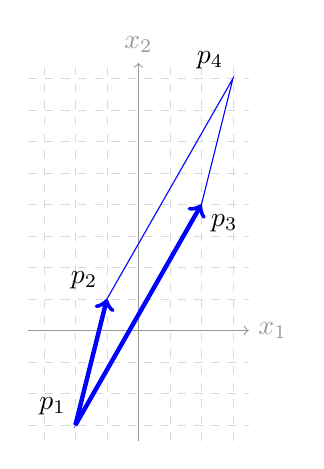
\begin{tikzpicture}[scale=0.4]
\def\XMAX{3.5};\def\YMAX{8.5};
\draw[help lines, color=gray!30, dashed] (-\XMAX,-\YMAX+5) grid (\XMAX,\YMAX);
\draw[->, color=gray!80] (-\XMAX,0)--(\XMAX,0) node[right]{$x_1$};
\draw[->, color=gray!80] (0,-\YMAX+5)--(0,\YMAX) node[above]{$x_2$};
\coordinate (p1) at (-2,-3); \node at (p1)[above left]{$p_1$};
\coordinate (p2) at (-1,1); \node at (p2)[above left]{$p_2$};
\coordinate (p3) at (2,4); \node at (p3)[below right]{$p_3$};
\coordinate (p4) at (3,8); \node at (p4)[above left]{$p_4$};
\draw[blue] (p1)--(p2)--(p4)--(p3)--cycle;
\draw[->,ultra thick,blue] (p1)--(p2);
\draw[->,ultra thick,blue] (p1)--(p3);
\end{tikzpicture}
\end{center}
\end{solution}

\begin{problem}
$\det(A-B)=\det A-\det B$
\end{problem}

\begin{solution}
This is false, for example, we could just take $A=I=\begin{bmatrix}
1&0\\0&1
\end{bmatrix}$, $B=-I$, then $4=\det(2I)=\det(A-B)\neq \det A-\det B=1-1=0$
\end{solution}

\begin{problem}
If $A$ is a 3 by 3 matrix, then $\det(2A)=8(\det A)$
\end{problem}

\begin{solution}
This is true.
\end{solution}

\begin{problem}
Suppose $A,B$ are both 3 by 3 matrices, and $\det A=2$, $\det B=\frac{1}{3}$, then the determinant of $A^TB^{-1}$ is
\end{problem}

\begin{solution}
$\det(A^TB^{-1})=\det(A^T)\det(B^{-1})=(\det A)(\det B)^{-1}=2\cdot 3=6$.
\end{solution}

\begin{problem}
Suppose $A$ is a 3 by 3 matrix with entries integers, and $A^3=I$ is the identity matrix. Then the determinant of $A$ has to be
\end{problem}

\begin{solution}
$\det A$ must be some real number. $1=\det I=\det(A^3)=(\det A)^3\Rightarrow \det A=\sqrt[3]{1}=1$.
\end{solution}

\subsection{Online Assignment 6}

\begin{problem}
Suppose $A=\begin{bmatrix}
1&2&1&2&-1&3\\
0&0&0&0&1&-1\\
0&0&1&3&1&-2\\
\end{bmatrix}$
\begin{enumerate}[label=\alph*)]
\item Find a basis for the null space of $A$
\item Find a basis for the column space of $A$
\item Find a basis for the row space of $A$
\end{enumerate}
\end{problem}

\begin{solution}
First realize
\[
A\xsim{R2\leftrightarrow R3}\begin{bmatrix}
1&2&1&2&-1&3\\
0&0&1&3&1&-2\\
0&0&0&0&1&-1\\
\end{bmatrix}\sim\begin{bmatrix}
1&2&0&-1&0&3\\
0&0&1&3&0&-1\\
0&0&0&0&1&-1\\
\end{bmatrix}
\]
Hence the solution in parametric form is $x_2\begin{bmatrix}
-2\\1\\0\\0\\0\\0
\end{bmatrix}+x_4\begin{bmatrix}
1\\0\\-3\\1\\0\\0
\end{bmatrix}+x_6\begin{bmatrix}
-3\\0\\1\\0\\1\\1
\end{bmatrix}$. And the pivot columns are the 1st, 3rd and 5th columns
\begin{enumerate}[label=\alph*)]
\item A basis for $\Nul A$ could be $\left\{\begin{bmatrix}
-2\\1\\0\\0\\0\\0
\end{bmatrix},\begin{bmatrix}
1\\0\\-3\\1\\0\\0
\end{bmatrix},\begin{bmatrix}
-3\\0\\1\\0\\1\\1
\end{bmatrix}\right\}$
\item A basis for $\Col A$ could be $\left\{\begin{bmatrix}
1\\0\\0
\end{bmatrix},\begin{bmatrix}
1\\0\\1
\end{bmatrix},\begin{bmatrix}
-1\\1\\1
\end{bmatrix}\right\}$
\item A basis for $\Row A$ could be
\[
\left\{\begin{bmatrix}
1&2&0&-1&0&3
\end{bmatrix},\begin{bmatrix}
0&0&1&3&0&-1
\end{bmatrix},\begin{bmatrix}
0&0&0&0&1&-1
\end{bmatrix}\right\}
\]
\end{enumerate}
\end{solution}

\begin{problem}
Suppose $A=\begin{bmatrix}
3&-1&-5\\
1&1&-1\\
-2&2&4\\
\end{bmatrix}$
\begin{enumerate}[label=\alph*)]
\item Determine whether $\mathbf u=\begin{bmatrix}
-3\\1\\-2
\end{bmatrix}$ is in the null space of $A$. Explain your reasoning.
\item Determine whether $\mathbf b=\begin{bmatrix}
1\\-3\\-4
\end{bmatrix}$ is in the column space of $A$. Explain your reasoning.
\end{enumerate}
\end{problem}

\begin{solution}
\begin{enumerate}[label=\alph*)]
\item $\mathbf u\in\Nul A$ since $A\mathbf u=\mathbf0$
\item $\mathbf b\in\Col A$ since linear system $A\mathbf x=\mathbf b$ is consistent
\end{enumerate}
\end{solution}

\begin{problem}
Recall $\mathbb P_2=\{a_0+a_1t+a_2t^2|a_0,a_1,a_2\in\mathbb R\}$ is the set of polynomials of degree less or equal to 2. Let $V$ be the subset of $\mathbb P_2$ consists of polynomials that evalute to 0 at $t=1$ (i.e. polynomial $p(t)$ is in $V$ if $p(1)=0$ and of degree less or equal to 2). With the usual addition and scalar multiplication for polynomials
\begin{enumerate}[label=\alph*)]
\item Show that $V$ is a subspace.
\item Find a basis of $V$.
\item Cosider $T:V\to\mathbb R^2$ that maps polynomial $p(t)$ to $\begin{bmatrix}
p(-1)\\p(2)
\end{bmatrix}$, show $T$ is a linear transformation
\end{enumerate}
\end{problem}

\begin{solution}
\begin{enumerate}[label=\alph*)]
\item Realize that $V=\ker S$ for the linear transformation $S:\mathbb P_2\to\mathbb R$, $S(a_0+a_1t+a_2t^2)=a_0+a_1+a_2$, thus $V$ is a subspace of $\mathbb P_2$
\item This is precisely Example~\ref{10:24-07/01/2022}
\item For any $p(t),q(t)\in V$ and $c\in\mathbb R$, we have
\[
T(p+q)=\begin{bmatrix}
(p+q)(-1)\\(p+q)(2)
\end{bmatrix}=\begin{bmatrix}
p(-1)+q(-1)\\p(2)+q(2)
\end{bmatrix}=\begin{bmatrix}
p(-1)\\p(2)
\end{bmatrix}+\begin{bmatrix}
q(-1)\\q(2)
\end{bmatrix}=T(p)+T(q)
\]
\[
T(cp)=\begin{bmatrix}
(cp)(-1)\\(cp)(2)
\end{bmatrix}=\begin{bmatrix}
c\cdot p(-1)\\c\cdot p(2)
\end{bmatrix}=c\begin{bmatrix}
p(-1)\\p(2)
\end{bmatrix}=cT(p)
\]
Therefore $T:V\to\mathbb R^2$ is a linear transformation
\end{enumerate}
\end{solution}

\begin{problem}
We say a square matrix $A$ is \textcolor{blue}{anti-symmetric}\index{anti-symmetric} if $A^T=-A$. Denote the set of $3\times3$ anti-symmetric matrices $V$.
\begin{enumerate}[label=\alph*)]
\item Show that $V$ is a vector space.
\item What is the dimension of $V$?
\item Find a basis of $V$.
\item Show that
\[
\mathcal B=\left\{B_1=\begin{bmatrix}
0&-1&-1\\
1&0&-1\\
1&1&0\\
\end{bmatrix},B_2=\begin{bmatrix}
0&2&0\\
-2&0&-1\\
0&1&0\\
\end{bmatrix},B_3=\begin{bmatrix}
0&-1&-2\\
1&0&-3\\
2&3&0\\
\end{bmatrix}\right\}
\]
form a basis for $V$.
\end{enumerate}
\end{problem}

\begin{solution}
\begin{enumerate}[label=\alph*)]
\item For any $A,B\in V$ and $c\in\mathbb R$, by definition $A^T=-A, B^T=-B$, so
\[
(A+B)^T=A^T+B^T=-A-B=-(A+B)
\]
\[
(cA)^T=cA^T=c(-A)=-(cA)
\]
hence $A+B,cA\in V$, i.e. $V$ is a closed under addition and scalar multiplication. Therefore $V$ is a subspace of $M_{3\times2}(\mathbb R)$, and consequently a vector space.
\item It is not hard to realize
\[
V=\left\{\begin{bmatrix}
0&-a&-b\\
a&0&-c\\
b&c&0
\end{bmatrix}\in\ M_{3\times3}(\mathbb R)\middle|a,b,c\in\mathbb R\right\}\cong\mathbb R^3
\]
Thus $\dim V=3$
\item Note that
\begin{equation}\label{14:56-06/24/2022}
\begin{aligned}
\begin{bmatrix}
0&-a&-b\\
a&0&-c\\
b&c&0
\end{bmatrix}&=\begin{bmatrix}
0&-a&0\\
a&0&0\\
0&0&0
\end{bmatrix}+\begin{bmatrix}
0&0&-b\\
0&0&0\\
b&0&0
\end{bmatrix}+\begin{bmatrix}
0&0&0\\
0&0&-c\\
0&c&0
\end{bmatrix}\\
&=a\begin{bmatrix}
0&-1&0\\
1&0&0\\
0&0&0
\end{bmatrix}+b\begin{bmatrix}
0&0&-1\\
0&0&0\\
1&0&0
\end{bmatrix}+c\begin{bmatrix}
0&0&0\\
0&0&-1\\
0&1&0
\end{bmatrix}
\end{aligned}
\end{equation}
So we know that
\[
\mathcal E=\{E_1,E_2,E_3\}=
\left\{
\begin{bmatrix}
0&-1&0\\
1&0&0\\
0&0&0
\end{bmatrix},\begin{bmatrix}
0&0&-1\\
0&0&0\\
1&0&0
\end{bmatrix},\begin{bmatrix}
0&0&0\\
0&0&-1\\
0&1&0
\end{bmatrix}\right\}
\]
is a basis for $V$, this is linearly independent since the linear combination \eqref{14:56-06/24/2022} is equal to zero $\iff a=b=c=0$
\item The coordinate vectors $\{[B_1]_{\mathcal E},[B_2]_{\mathcal E},[B_3]_{\mathcal E}\}=\left\{\begin{bmatrix}
1\\1\\0
\end{bmatrix},\begin{bmatrix}
1\\0\\1
\end{bmatrix},\begin{bmatrix}
0\\1\\1
\end{bmatrix}\right\}$ form a basis for $\mathbb R^3$, so $\mathcal B$ form a basis for $V$
\end{enumerate}
\end{solution}

\subsection{Online Assignment 7}

\begin{problem}
Suppose $\mathbf v$ is an eigenvector for matrices $A$ and $B$, then $\mathbf v$ is an eigenvector for $A+B$ and $AB$.
\end{problem}

\begin{solution}
This is true. Since $\mathbf v$ is an eigenvector for both $A$ and $B$, there exist eigenvalues $\lambda_1,\lambda_2$ such that $A\mathbf v=\lambda_1\mathbf v$, $B\mathbf v=\lambda_2\mathbf v$, so we have $(A+B)\mathbf v=A\mathbf v+B\mathbf v=\lambda_1\mathbf v+\lambda_2\mathbf v=(\lambda_1+\lambda_2)\mathbf v$. In other words, $\mathbf v$ is an eigenvector for $A+B$ with eigenvalue $\lambda_1+\lambda_2$. Similarly, we also have $AB\mathbf v=A(\lambda_1\mathbf v_1)=\lambda_2 A\mathbf v=\lambda_1\lambda_2\mathbf v$. In other words, $\mathbf v$ is an eigenvector for $AB$ with eigenvector $\lambda_1\lambda_2$
\end{solution}

\begin{problem}
Suppose $t+3t^2-2t^3$ is the characteristic polynomial of a 3 by 3 matrix, then $A$ is not invertible.
\end{problem}

\begin{solution}
This is true. Note that $t=0$ is a root of the characteristic polynomial, so the null space of $A$ is not trivial, $A$ is not invertible.
\end{solution}

\begin{problem}
Suppose $\mathcal B=\left\{1+t,1+2t^2,1-t+t^2\right\}$ and $\mathcal C=\left\{1-t,t,t^2\right\}$ are two bases for $\mathbb P_2$, What is the change of basis matrix $\underset{\mathcal C\leftarrow\mathcal B}{P}$ from $\mathcal B$ to $\mathcal C$. Please show all your work.
\end{problem}

\begin{solution}
First let's find the change of basis matrices from $\mathcal B$ and $\mathcal C$ to the standard basis $\mathcal E=\{1,t,t^2\}$. We have
\[
\underset{\mathcal E\leftarrow\mathcal B}{P}=\begin{bmatrix}
[1+t]_{\mathcal E}&[1+2t^2]_{\mathcal E}&[1-t+t^2]_{\mathcal E}
\end{bmatrix}=\begin{bmatrix}
1&1&1\\
1&0&-1\\
0&2&1
\end{bmatrix}
\]
And
\[
\underset{\mathcal E\leftarrow\mathcal C}{P}=\begin{bmatrix}
[1-t]_{\mathcal E}&[t]_{\mathcal E}&[t^2]_{\mathcal E}
\end{bmatrix}=\begin{bmatrix}
1&0&0\\
-1&1&0\\
0&0&1
\end{bmatrix}
\]
Hence we have
\begin{align*}
\underset{\mathcal C\leftarrow\mathcal B}{P}=\left(\underset{\mathcal C\leftarrow\mathcal E}{P}\right)\left(\underset{\mathcal E\leftarrow\mathcal B}{P}\right)=\left(\underset{\mathcal E\leftarrow\mathcal C}{P}\right)^{-1}\left(\underset{\mathcal E\leftarrow\mathcal B}{P}\right)=\begin{bmatrix}
1&0&0\\
-1&1&0\\
0&0&1
\end{bmatrix}^{-1}\begin{bmatrix}
1&1&1\\
1&0&-1\\
0&2&1
\end{bmatrix}=\begin{bmatrix}
1       &       1  &            1       \\
2        &      1 &             0       \\
0         &     2&              1 
\end{bmatrix}
\end{align*}
\end{solution}

\begin{problem}
If $Nul A$ is 2-dimensional, then $0$ is an eigenvalue of $A$.
\end{problem}

\begin{solution}
This is true. Since if $\Nul A$ is 2-dimensional, then $\Nul A$ is non-trivial, thus $0$ is an eigenvalue of $A$
\end{solution}

\begin{problem}
Is $\begin{bmatrix}0\\0\\1\end{bmatrix}$ an eigenvector of $\begin{bmatrix}2&0&0\\3&2&0\\0&4&3\end{bmatrix}$? If so, find the corresponding eigenvalue, if not, please explain why.
\end{problem}

\begin{solution}
Note that $\begin{bmatrix}2&0&0\\3&2&0\\0&4&3\end{bmatrix}\begin{bmatrix}0\\0\\1\end{bmatrix}=\begin{bmatrix}0\\0\\3\end{bmatrix}$. so $\begin{bmatrix}0\\0\\1\end{bmatrix}$ is an eigenvector with eigenvalue 3
\end{solution}

\begin{problem}
Find all eigenvalues of $A=\begin{bmatrix}6&-2&0\\-2&9&0\\5&8&3\end{bmatrix}$. Please show all your work.
\end{problem}

\begin{solution}
\begin{align*}
\left|tI-A\right|&=\left|\begin{matrix}
t-6&2&0\\
2&t-9&0\\
-5&-8&t-3
\end{matrix}\right|\xequal{\text{cofator expansion across 3rd column}}(t-3)(-1)^{3+3}\left|\begin{matrix}
t-6&2\\
2&t-9
\end{matrix}\right|\\
&=(t-3)((t-6)(t-9)-2\cdot 2)=(t-3)(t^2-5t+50)=(t-3)(t-5)(t-10)
\end{align*}
Therefore eigenvalues for $A$ are 3,5,10.
\end{solution}

\begin{problem}
Assume that $A$ is similar to an upper triangular matrix $U$, then $\det A$ is the product of all its eigenvalues (counting multiplicity). Please explain why.
\end{problem}

\begin{solution}
Suppose the diagonal elements of $A$ are $\lambda_1,\cdots,\lambda_n$, then the charateristic polynomial of $A$ is the same the charateristic polynomial $U$ (Since they are similar) which would be $(t-\lambda_1)\cdots(t-\lambda_n)$, so $\lambda_1,\cdots,\lambda_n$ are the eigenvalues for $A$. And the determinant of $A$ is the same as the determinant of $U$ (Since they are similar) which is $\lambda_1\cdots\lambda_n$
\end{solution}

\subsection{Online Assignment 8}

\begin{problem}
Suppose $A=\begin{bmatrix}
2&2&1\\
1&3&1\\
1&2&2
\end{bmatrix}$, determine whether $A$ is diagonalizable. If it is, please find a diagonalization. If not, please explain why.
\end{problem}

\begin{solution}
First we evaluate the characteristic polynomial of $A$
\begin{align*}
\det(tI-A)&=\left|\begin{matrix}
t-2&-2&-1\\
-1&t-3&-1\\
-1&-2&t-2
\end{matrix}\right|\xequal{\substack{R1\rightarrow R1+(t-2)R3\\R2\rightarrow R2-R3}}\left|\begin{matrix}
0&-2(t-1)&(t-1)(t-3)\\
0&t-1&-(t-1)\\
-1&-2&t-2
\end{matrix}\right|\\
&\xequal{\text{factor out $(t-1)$ on row 1 and row 2}}(t-1)^2\left|\begin{matrix}
0&-2&(t-3)\\
0&1&-1\\
-1&-2&t-2
\end{matrix}\right|=(t-1)^2(t-5)
\end{align*}
So the eigenvalues are $\lambda_1=\lambda_2=1$, $\lambda_3=5$. For the 1-eigenspace, we consider
\begin{align*}
\left[\begin{array}{c|c}
I-A&\mathbf0
\end{array}\right]&=
\left[\begin{array}{ccc|c}
-1&-2&-1&0\\
-1&-2&-1&0\\
-1&-2&-1&0
\end{array}\right]\sim\left[\begin{array}{ccc|c}
1&2&1&0\\
0&0&0&0\\
0&0&0&0
\end{array}\right]
\end{align*}
So we get two basis vectors $\left\{\mathbf v_1=\begin{bmatrix}
-2\\1\\0
\end{bmatrix},\mathbf v_2=\begin{bmatrix}
-1\\0\\1
\end{bmatrix}\right\}$. For the 5-eigenspace, we consider
\begin{align*}
\left[\begin{array}{c|c}
5I-A&\mathbf0
\end{array}\right]&=
\left[\begin{array}{ccc|c}
3&-2&-1&0\\
-1&2&-1&0\\
-1&-2&3&0
\end{array}\right]\sim\left[\begin{array}{ccc|c}
1&0&-1&0\\
0&1&-1&0\\
0&0&0&0
\end{array}\right]
\end{align*}
So we get a basis vector $\left\{\mathbf v_3=\begin{bmatrix}
1\\1\\1
\end{bmatrix}\right\}$
\item From above, we get the diagonalization
\[
A=PDP^{-1}=\begin{bmatrix}
-2&-1&1\\
1&0&1\\
0&1&1
\end{bmatrix}\begin{bmatrix}
1&0&0\\
0&1&0\\
0&0&5
\end{bmatrix}\begin{bmatrix}
-\frac{1}{4}&\frac{1}{2}&-\frac{1}{4}\\
-\frac{1}{4}&-\frac{1}{2}&\frac{3}{4}\\
\frac{1}{4}&\frac{1}{2}&\frac{1}{4}
\end{bmatrix}
\]
\end{solution}

\begin{problem}
Suppose $A=\begin{bmatrix}
-6&8\\
-4&6
\end{bmatrix}$, Please evaluate $A^{101}$, show all your work.
\end{problem}

\begin{solution}
First we can diagonalize $A$ as
\[
A=\begin{bmatrix}
1&2\\
1&1
\end{bmatrix}\begin{bmatrix}
2&0\\
0&-2
\end{bmatrix}\begin{bmatrix}
-1&2\\
1&-1
\end{bmatrix}
\]
\[
A^{101}=PD^{101}P^{-1}=\begin{bmatrix}
1&2\\
1&1
\end{bmatrix}\begin{bmatrix}
2^{101}&0\\
0&-2^{101}
\end{bmatrix}\begin{bmatrix}
-1&2\\
1&-1
\end{bmatrix}
\]
\end{solution}

\begin{problem}
Suppose $T:\mathbb R^3\to\mathbb R^3$ is a linear transformation, $\mathcal B=\{\mathbf b_1,\mathbf b_2,\mathbf b_3\}$, $\mathcal C=\{\mathbf c_1,\mathbf c_2,\mathbf c_3\}$ are two different bases for $\mathbb R^3$. Determine whether the following is possible.
\begin{enumerate}[label=\alph*)]
\item $[T]_{\mathcal B}=\begin{bmatrix}
1 &2&4\\
3 &-1 &-2\\
2 &-1& 3
\end{bmatrix}$ and $[T]_{\mathcal C}=\begin{bmatrix}
1& -3 &1\\
2 &1& 6\\
0 &3 &8
\end{bmatrix}$
\item $[T]_{\mathcal B}=\begin{bmatrix}
3&0&0\\
2&2&0\\
2&3&4
\end{bmatrix}$ and $[T]_{\mathcal C}=\begin{bmatrix}
1&-1&0\\
2&4&0\\
3&-2&4
\end{bmatrix}$
\end{enumerate}
\end{problem}

\begin{solution}
\begin{enumerate}[label=\alph*)]
\item This is not possible since these two matrices have different determinant.
\item This is possible since these two matrix has the same the characteristic polynomial $(t-2)(t-3)(t-4)$, hence they are similar to same diagonal matrix, and thus similar.
\end{enumerate}
\end{solution}

\begin{problem}
Suppose $A$ is similar to $B$.
\begin{enumerate}[label=\alph*)]
\item Could you conclude that $3A$ is similar to $3B$. If you can, please give your reasons, if not, please find a counter-example.
\item Could you conclude that $A^{-1}$ is similar to $B^{-1}$. If you can, please give your reasons, if not, please find a counter-example.
\end{enumerate}
\end{problem}

\begin{solution}
Since $A$ is similar to $B$, we may assume $A=PBP^{-1}$.
\begin{enumerate}[label=\alph*)]
\item $3A=3PBP^{-1}=P(3B)P^{-1}$ is similar.
\item $A^{-1}=(PBP^{-1})^{-1}=PB^{-1}P^{-1}$ is similar.
\end{enumerate}
\end{solution}

\subsection{Online Assignment 9}

\begin{problem}
Determine whether the following statements are true
\begin{enumerate}[label=\alph*)]
\item $\|\mathbf u\|^2+\|\mathbf v\|^2=\|\mathbf u+\mathbf v\|^2$ if and only if $\mathbf u,\mathbf v$ are orthogonal.
\item If $W$ is a subspace of $\mathbb R^n$, and vector $\mathbf v$ is orthogonal to both $W$ and $W^\perp$, then $\mathbf v=\mathbf0$.
\item If $W = \Span\{\mathbf x_1, \mathbf x_2 ,\mathbf x_3\}$ with $\{\mathbf x_1, \mathbf x_2 ,\mathbf x_3\}$ linearly independent, and if $\{\mathbf v_1, \mathbf v_2 ,\mathbf v_3\}$ is an orthogonal set in $W$, then $\{\mathbf v_1, \mathbf v_2 ,\mathbf v_3\}$ is a basis for $W$.
\end{enumerate}
\end{problem}

\begin{solution}
\begin{enumerate}[label=\alph*)]
\item This is true. $\|\mathbf u+\mathbf v\|^2=(\mathbf u+\mathbf v)\cdot(\mathbf u+\mathbf v)=\mathbf u\cdot\mathbf u+2\mathbf u\cdot\mathbf v+\mathbf v\cdot\mathbf v=\|\mathbf u\|^2+\|\mathbf v\|^2+2\mathbf u\cdot\mathbf v$. Thus the equality holds $\iff\mathbf u\cdot\mathbf v=0$, i.e. $\mathbf u,\mathbf v$ are orthogonal.
\item Consider $\mathbf v\cdot\mathbf v=\|\mathbf v\|^2$, it should be 0 since $\mathbf v$ is in both $W$ and $W^\perp$, so $\mathbf v=\mathbf 0$
\item This is true by Theorem~\ref{01:12-07/15/2022}
\end{enumerate}
\end{solution}

\begin{problem}
Suppose $A=\begin{bmatrix}
1&2&3\\
2&1&-1\\
0&2&4\\
3&5&-1
\end{bmatrix}$, please find a basis for $(\Col A)^\perp$.
\end{problem}

\begin{solution}
Recall that $(\Col A)^\perp=\Nul(A^T)$. And we can find a basis for $\Nul(A^T)$ through
\[
\left[\begin{array}{c|c}
A^T&\mathbf0
\end{array}\right]=\left[\begin{array}{cccc|c}
1&2&0&3&0\\
2&1&2&5&0\\
3&-1&4&1&0
\end{array}\right]\sim\left[\begin{array}{cccc|c}
1&0&0&-13&0\\
0&1&0&8&0\\
0&0&1&\frac{23}{2}&0
\end{array}\right]
\]
Thus
\[
(\Col A)^\perp=\Span\left\{\begin{bmatrix}
13\\-8\\-\frac{23}{2}\\1
\end{bmatrix}\right\}
\]
\end{solution}

\begin{problem}
Suppose we have $\mathcal B=\left\{\mathbf u_1=\begin{bmatrix}1\\1\\0\\-1\end{bmatrix},\mathbf u_2=\begin{bmatrix}1\\0\\1\\1\end{bmatrix},\mathbf u_3=\begin{bmatrix}0\\-1\\1\\-1\end{bmatrix}\right\}$, please justify that $\mathcal B$ is an orthogonal set, suppose $\mathbf y=\begin{bmatrix}1\\2\\3\\4\end{bmatrix}$, $L$ is the subspace spanned by $\mathcal B$, compute the projection $\Proj_L\mathbf y$ of $\mathbf y$ onto $L$.
\end{problem}

\begin{solution}
Let $A=\begin{bmatrix}
\mathbf u_1&\mathbf u_2&\mathbf u_3
\end{bmatrix}=\begin{bmatrix}
1&1&0\\
1&0&-1\\
0&1&1\\
-1&1&-1
\end{bmatrix}$, we can check that $A^TA=I$ is the 3 by 3 identity matrix, so $\mathcal B$ is an orthogonal set. And therefore
\begin{align*}
\Proj_L\mathbf y&=\frac{\mathbf y\cdot\mathbf u_1}{\mathbf u_1\cdot\mathbf u_1}\mathbf u_1+\frac{\mathbf y\cdot\mathbf u_2}{\mathbf u_2\cdot\mathbf u_2}\mathbf u_2+\frac{\mathbf y\cdot\mathbf u_3}{\mathbf u_3\cdot\mathbf u_3}\mathbf u_3\\
&=\frac{-1}{3}\mathbf u_1+\frac{8}{3}\mathbf u_2+\frac{-3}{3}\mathbf u_3\\
&=-\frac{1}{3}\begin{bmatrix}
1\\1\\0\\-1
\end{bmatrix}+\frac{8}{3}\begin{bmatrix}
1\\0\\1\\1
\end{bmatrix}-\begin{bmatrix}
0\\-1\\1\\-1
\end{bmatrix}=\begin{bmatrix}
\frac{7}{3}\\\frac{2}{3}\\\frac{5}{3}\\4
\end{bmatrix}
\end{align*}
\end{solution}

\begin{problem}
Suppose $A=\begin{bmatrix}
-1&6&6\\
3&-8&3\\
1&-2&6\\
1&-4&-3
\end{bmatrix}$, please find an orthogonal basis for $\Col A$.
\end{problem}

\begin{solution}
We apply the Gram-Schmidt process here
\begin{itemize}
\item $\mathbf u_1=\mathbf v_1=\begin{bmatrix}
-1\\3\\1\\1
\end{bmatrix}$
\item $\mathbf u_2=\mathbf v_2-\dfrac{\mathbf v_2\cdot\mathbf u_1}{\mathbf u_1\cdot\mathbf u_1}\mathbf u_1=\begin{bmatrix}
6\\-8\\-2\\-4
\end{bmatrix}-\frac{-36}{12}\begin{bmatrix}
-1\\3\\1\\1
\end{bmatrix}=\begin{bmatrix}
3\\1\\1\\-1
\end{bmatrix}$
\item $\mathbf u_3=\mathbf v_3-\dfrac{\mathbf v_3\cdot\mathbf u_1}{\mathbf u_1\cdot\mathbf u_1}\mathbf u_1-\dfrac{\mathbf v_3\cdot\mathbf u_2}{\mathbf u_2\cdot\mathbf u_2}\mathbf u_2=\begin{bmatrix}
6\\3\\6\\-3
\end{bmatrix}-\frac{6}{12}\begin{bmatrix}
-1\\3\\1\\1
\end{bmatrix}-\frac{30}{12}\begin{bmatrix}
3\\1\\1\\-1
\end{bmatrix}=\begin{bmatrix}
-1\\-1\\3\\-1
\end{bmatrix}$
\end{itemize}
So we have an orthogonal basis for $\Col A$
\[
\Col A=\Span\left\{\begin{bmatrix}
-1\\3\\1\\1
\end{bmatrix},\begin{bmatrix}
3\\1\\1\\-1
\end{bmatrix},\begin{bmatrix}
-1\\-1\\3\\-1
\end{bmatrix}\right\}
\]
\end{solution}

\subsection{Online Assignment 10}

\begin{problem}
Determine whether the following statements are correct
\begin{enumerate}[label=\alph*)]
\item If $A$ is symmetric and if vectors $\mathbf u$ and $\mathbf v$ such that $A\mathbf u = \mathbf u$ and $\mathbf v$ is in $\operatorname{Nul}A$, then $\mathbf u \cdot\mathbf v = \mathbf0$.
\item $\operatorname{Nul}A=\operatorname{Nul}A^TA$.
\end{enumerate}
\end{problem}

\begin{solution}
\begin{enumerate}[label=\alph*)]
\item The eigenvalues for eigenvectors $\mathbf u$ and $\mathbf v$ are 1 and 0, and $A$ is symmetric, by Theorem~\ref{23:54-07/19/2022}, $\mathbf u\cdot\mathbf v=0$.
\item If $\mathbf x\in\Nul A$, then $A\mathbf x=\mathbf0$, so $A^TA\mathbf x=\mathbf 0$. If $\mathbf x\in\Nul(A^TA)$, then $A^TA\mathbf x=\mathbf0$, so $0=\mathbf x^TA^TA\mathbf x=\|A\mathbf x\|^2$, so $A\mathbf x=0$.
\end{enumerate}
\end{solution}

\begin{problem}
Find the least-squares solution(s) to $\begin{bmatrix}
1&5\\
3&1\\
-2&4
\end{bmatrix}\begin{bmatrix}
x_1\\x_2
\end{bmatrix}=\begin{bmatrix}
4\\-2\\-3
\end{bmatrix}$.
\end{problem}

\begin{solution}
Let's denote $A=\begin{bmatrix}
1&5\\
3&1\\
-2&
\end{bmatrix}$, $\mathbf b=\begin{bmatrix}
4\\-2\\-3
\end{bmatrix}$, then $A^TA=\begin{bmatrix}
14&0\\
0&42
\end{bmatrix}$, and $A^T\mathbf b=\begin{bmatrix}
4\\6
\end{bmatrix}$, then we get the least -square solution $\hat{\mathbf x}=(A^TA)^{-1}A^T\mathbf b=\begin{bmatrix}
\frac{2}{7}\\\frac{1}{7}
\end{bmatrix}$
\end{solution}

\begin{problem}
Orthogonal diagonalize the matrix $\begin{bmatrix}
3&4\\
4&9
\end{bmatrix}$.
\end{problem}

\begin{solution}
First note that $A=\begin{bmatrix}
3&4\\
4&9
\end{bmatrix}$ is symmetric and real-valued, we can get its eigenvalues $\lambda_1=1$, $\lambda_2=11$, and normalized eigenvectors $\mathbf u_1=\begin{bmatrix}
-\frac{2}{\sqrt5}\\\frac{1}{5}
\end{bmatrix}$, $\mathbf u_2=\begin{bmatrix}
\frac{1}{5}\\\frac{2}{5}
\end{bmatrix}$. Hence we have the orthogonal diganolization
\[
A=\begin{bmatrix}
3&4\\
4&9
\end{bmatrix}=\begin{bmatrix}
-\frac{2}{\sqrt5}&\frac{1}{\sqrt5}\\
\frac{1}{5}&\frac{2}{\sqrt5}
\end{bmatrix}\begin{bmatrix}
1&0\\0&11
\end{bmatrix}\begin{bmatrix}
-\frac{2}{\sqrt5}&\frac{1}{\sqrt5}\\
\frac{1}{5}&\frac{2}{\sqrt5}
\end{bmatrix}=PDP^T
\]
\end{solution}

\begin{problem}
Suppose $A=\begin{bmatrix}
1&5\\
-2&3
\end{bmatrix}$.
\begin{enumerate}[label=\alph*)]
\item Please find the eigenvalues of $A$.
\item Please find the eigenvectors of $A$.
\item Please write $A$ as matrix multiplication $PCP^{-1}$, where $C$ is of the form $\begin{bmatrix}
a&-b\\
b&c
\end{bmatrix}$.
\end{enumerate}
\end{problem}

\begin{solution}
\begin{enumerate}[label=\alph*)]
\item The characteristic polynomial is $t^2-4t13$, and so the eigenvalues are $\lambda=2-3i$, $\overline\lambda=2+3i$, so we have $a=2$, $b=3$ and $C=\begin{bmatrix}
2&-3\\3&2
\end{bmatrix}$
\item The eigenvalues for $\lambda,\overline{\lambda}$ are $\mathbf v=\begin{bmatrix}
1+3i\\2
\end{bmatrix}=\begin{bmatrix}
1\\2
\end{bmatrix}+i\begin{bmatrix}
3\\0
\end{bmatrix}$, $\overline{\mathbf v}=\begin{bmatrix}
1-3i\\2
\end{bmatrix}$. so $P=\begin{bmatrix}
1&3\\
2&0
\end{bmatrix}$
\item From above computation we get decomposition
\[
A=\begin{bmatrix}
1&3\\
2&0
\end{bmatrix}\begin{bmatrix}
2&-3\\3&2
\end{bmatrix}\begin{bmatrix}
0&\frac{1}{2}\\
\frac{1}{3}&-\frac{1}{6}
\end{bmatrix}=PCP^{-1}
\]
\end{enumerate}
\end{solution}

\end{document}